\let\negmedspace\undefined
\let\negthickspace\undefined
\documentclass[journal]{IEEEtran}
\usepackage[a5paper, margin=10mm, onecolumn]{geometry}
%\usepackage{lmodern} % Ensure lmodern is loaded for pdflatex
\usepackage{tfrupee} % Include tfrupee package

\setlength{\headheight}{1cm} % Set the height of the header box
\setlength{\headsep}{0mm}     % Set the distance between the header box and the top of the text

\usepackage{gvv-book}
\usepackage{gvv}
\usepackage{cite}
\usepackage{amsmath,amssymb,amsfonts,amsthm}
\usepackage{algorithmic}
\usepackage{graphicx}
\usepackage{textcomp}
\usepackage{xcolor}
\usepackage{txfonts}
\usepackage{listings}
\usepackage{enumitem}
\usepackage{mathtools}
\usepackage{gensymb}
\usepackage{comment}
\usepackage[breaklinks=true]{hyperref}
\usepackage{tkz-euclide} 
\usepackage{listings}
% \usepackage{gvv}                                        
\def\inputGnumericTable{}                                 
\usepackage[latin1]{inputenc}                                
\usepackage{color}                                            
\usepackage{array}                                            
\usepackage{longtable}                                       
\usepackage{calc}                                             
\usepackage{multirow}                                         
\usepackage{hhline}                                           
\usepackage{ifthen}                                           
\usepackage{lscape}
\begin{document}

\bibliographystyle{IEEEtran}
\vspace{3cm}

\title{4.3.56}
\author{EE25BTECH11065 - Yoshita}
% \maketitle
% \newpage
% \bigskip
{\let\newpage\relax\maketitle}

\renewcommand{\thefigure}{\theenumi}
\renewcommand{\thetable}{\theenumi}
\setlength{\intextsep}{10pt} % Space between text and floats

\textbf{Question}:\\
Find the equation of the plane with intercepts 2, 3 and 4 on the x, y and z - axis respectively.\\
\bigskip

\textbf{Solution}:\\
The intercepts define three points on the plane, which we can label A, B, and C.
\begin{table}[H]    
  \centering
  \begin{table}[h!]
    \centering
    \begin{tabular}{|c|c|}
        \hline
        Point & Coordinates \\
        \hline
	    $A$ & $\myvec{1\\-1}$ \\
	    $B$ & $\myvec{-4\\2k}$ \\
	    $C$ & $\myvec{-k\\-5}$ \\
        \hline
    \end{tabular}
    \caption{Vertices of $\triangle ABC$ before substituting $k$}
    \label{tab:triangle_k}
\end{table}

  \caption{Answers}
  \label{Answers}
\end{table}
We can find two direction vectors, $\mathbf{m_1}$ and $\mathbf{m_2}$, that lie in the plane:
\begin{align*}
    \mathbf{m_1} &= \mathbf{B} - \mathbf{A} = \myvec{0-2\\3-0\\0-0} = \myvec{-2\\3\\0} \\
    \mathbf{m_2} &= \mathbf{C} - \mathbf{A} = \myvec{0-2\\0-0\\4-0} = \myvec{-2\\0\\4}
\end{align*}
The normal vector to the plane, $\mathbf{n}$, is found by the cross product of these two vectors.
\begin{align*}
    \mathbf{n} = \mathbf{m_1} \times \mathbf{m_2} &= \myvec{-2\\3\\0} \times \myvec{-2\\0\\4} \\
    &= \myvec{(3)(4) - (0)(0) \\ (0)(-2) - (-2)(4) \\ (-2)(0) - (3)(-2)} = \myvec{12\\8\\6}
\end{align*}
We can simplify the normal vector to $\mathbf{n} = \myvec{6\\4\\3}$. The equation of the plane is then given by:
\[ \mathbf{n}^T (\mathbf{x} - \mathbf{A}) = 0 \]
Substituting the numerical values, where $\mathbf{x} = [x, y, z]^T$:
\begin{align*}
    \myvec{6 & 4 & 3} \left( \myvec{x\\y\\z} - \myvec{2\\0\\0} \right) &= 0 \\
    \implies \myvec{6 & 4 & 3} \myvec{x-2\\y\\z} &= 0 \\
    \implies 6(x-2) + 4y + 3z &= 0 \\
    \implies 6x - 12 + 4y + 3z &= 0 \\
    \implies 6x + 4y + 3z &= 12
\end{align*}
\begin{figure}[h!]
\begin{center}
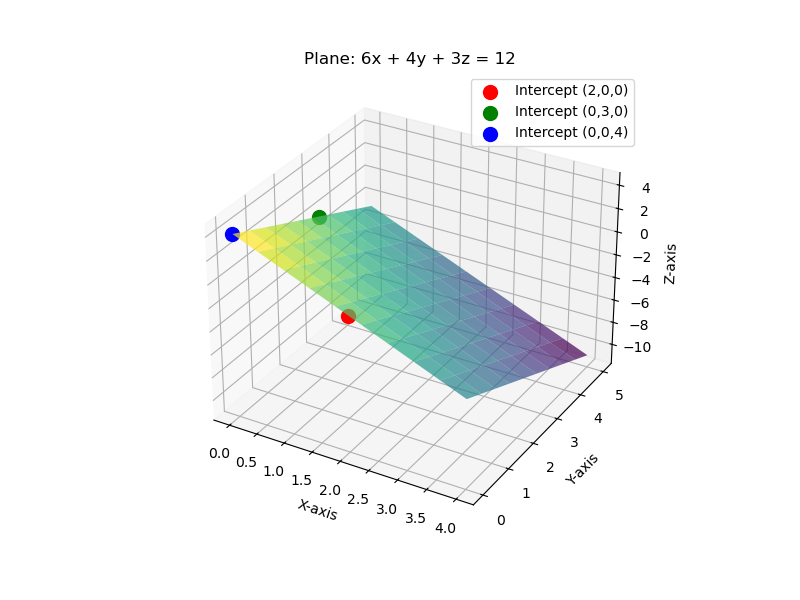
\includegraphics[width=0.9\columnwidth]{figs/fig2.png}
\end{center}
\caption{A plane intersecting the x, y, and z axes.}
\label{fig:Fig.1}
\end{figure}
\end{document}


